% !TEX root = ../example_paper.tex

\section{Hardware}
Z hárdverovej stránky sme potrebovali v tomto projekte vytvoriť dosku plošných spojov (PCB - Printed Circuit Boards) a návrh držiakov motorov, gyroskopu a kolies, ktorých výroba prebiehala pomocou 3D tlače.
\subsection{Model}
\label{sec:hardware}
Kolesá a ozubené koliesko pre hriadeľ motora boli vytlačené v 3D tlačiarni s resinovou náplňou FabPro 1000 Resin Cartridge Tough BLK. Na obrázkoch \ref{fig:gear} a \ref{fig:wheel_w_gear} môžeme vidieť návrhy ozubeného kolieska pre hriadeľ a kolesa. 

\begin{figure}[!htbp]
        \centering
        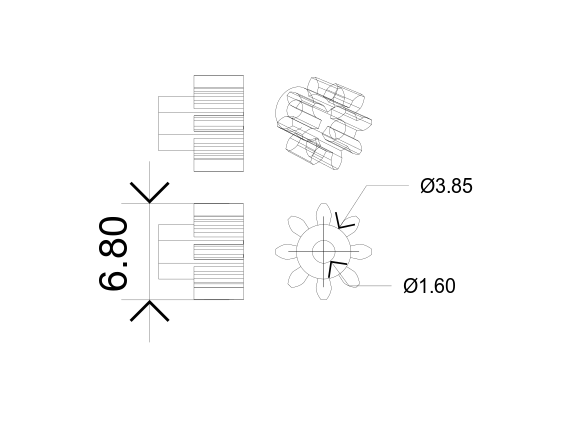
\includegraphics[scale=0.8]{includes/images/motor_gear.png}
        \caption{UTechnický nákres prevodu motora}
        \label{fig:gear}
\end{figure}

\begin{figure}[!htbp]
        \centering
        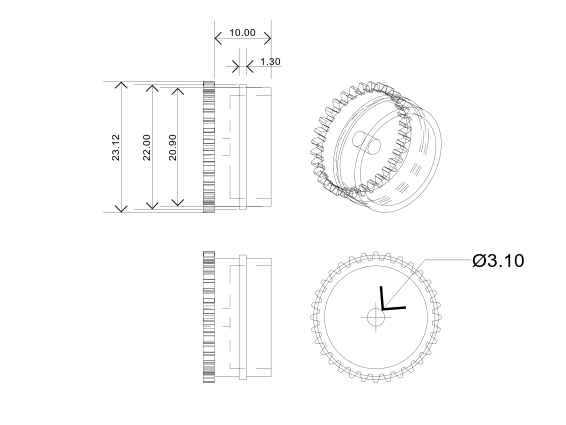
\includegraphics[scale=0.8]{includes/images/wheel_w_gear_2_blueprint.png}
        \caption{Koleso s prevodovkou}
        \label{fig:wheel_w_gear}
\end{figure}
\newpage
\subsection{Motory}\label{motor_section}
Použité motory boli vybrané s ohľadom na ich výkonnosť a spoľahlivosť. Sú to jednosmerné motory, vidieť ich môžeme na \ref{fig:motor} a detaily o nich uvádzame nižšie:

\begin{figure}[!htbp]
        \centering
        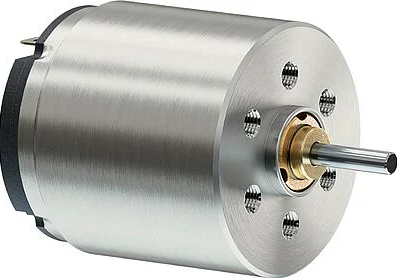
\includegraphics[scale=0.8]{includes/images/faulhaber.png}
        \caption{DC Mikromotor Faulhaber 1717T003SR}
        \label{fig:motor}
\end{figure}

\begin{itemize}
  \item Model: Faulhaber 1717 T 
  \item Typ: 003 SR
  \item Max. točivý moment: 5.35 mNm
  \item Max. rýchlosť: 11000 rpm
  \item Odkaz na technický list: \href{https://www.faulhaber.com/fileadmin/Import/Media/EN_1717_SR_DFF.pdf}{Technický list motora}
\end{itemize}

\subsection{Enkódery}\label{encoder_section}
Na monitorovanie polohy a otáčok motorov sme použili magnetické enkódery. Informáciu o rotácií získavajú ako zmenu magnetického poľa. Enkóder obsahuje dva Hallove články, ktoré merajú veľkosť magnetickej indukcie ako Hallovo napätie ako: 



\begin{equation}
\label{enc_eq}
U_H = h_H \frac{BI_p}{h}
\end{equation}
kde $U_H$ je Hallovo napätie, $h_H$ je Hallova konštanta, $B$ je magnetická indukcia, $I_p$ je pomocný prúd, $h$ je hrúbka polovodičovej doštičky. Tieto Hallove články merajú magnetickú indukciu v dvoch osiach na seba kolmých.



Enkóder obsahuje permanentný magnet pripevnený na jeho hriadeľ. Rotáciou hriadeľa sa točí magnet, a teda aj smer magnetického poľa. Zmeny v oboch osiach sú prekonvertované cez AD prevodník na digitálne signály. Skrz trigonometrické funkcie je následne vypočítaný fázový posun medzi týmito signálmi. To je dôležité nielen kvôli výpočtu rotácie hriadeľa, ale aj pre zistenie smeru rotácie.

Nižšie sú uvedené informácie o použitých enkóderoch \ref{fig:encoder}:

\begin{figure}[!htbp]
        \centering
        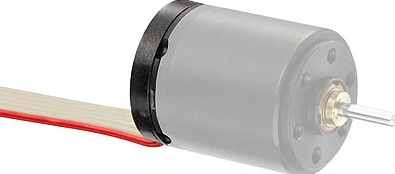
\includegraphics[scale=0.8]{includes/images/encoder.png}
        \caption{Enkóder IEH2-4096}
        \label{fig:encoder}
\end{figure}

\begin{itemize}
  \item Model: IEH2-4096
  \item Rozlíšenie: 4096
  \item Kanály: 2
  \item Odkaz na technický list: \href{https://www.faulhaber.com/fileadmin/Import/Media/EN_IEH2-4096_DFF.pdf}{Technický list enkódera}
\end{itemize}

\subsection{Gyroskop}

Na sledovanie orientácie a pohybu robota sme si zvolili MEMS gyroskop. Tie merajú uhlovú rýchlosť prostredníctvom Coriolisovho efektu. Coriolisova sila je spôsobená inerciou objektu v priamom pohybe, kolmo na smer pohybu objektu a jej výpočet je daný: 

\begin{equation}
\label{enc_eq}
\vec{F} = -2m\vec{\Omega_z}x\vec{v}
\end{equation}
MEMS Gyroskop obsahuje vybrujúce elementy na pružine. Keď sa gyroskop pohybuje kapacitný senzor deteguje vibrácie, tie sa následne premenia na uhlové zrýchlenie.
    \newpage
Ďalej sú uvedené podrobnosti o použitom module \ref{fig:gyro}:
\begin{figure}[!htbp]
        \centering
        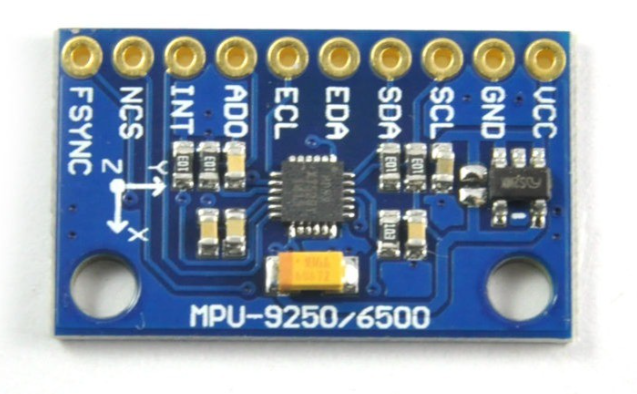
\includegraphics[scale=0.8]{includes/images/mpu9205.png}
        \caption{Gyroskop MPU9250}
        \label{fig:gyro}
\end{figure}
\begin{itemize}
  \item Model: MPU9250
  \item Typ: Gyroskop, akcelerometer a magnetometer
  \item Komunikácia: I2C, SPI
  \item Odkaz na technický list: \href{https://www.invensense.com/products/motion-tracking/9-axis/mpu-9250/}{MPU9250 Technical Datasheet}
\end{itemize}
\subsection{Laserový diaľkomer}
Ako vzdialenostný senzor sme zvolili Time-of-Flight (doba trvania letu) laserový merací modul poskytujúci presné meranie vzdialenosti bez ohľadu na farbu alebo odrazivosť cieľa. 
Time-of-Flight senzory fungujú na báze merania času letu laserového lúča vyslaného zo senzora, k objektu a naspäť. Vzdialenosť je z nameraného času vypočítaná podľa vzorca na \ref{tof_eq}:

\begin{equation}
\label{tof_eq}
d = \frac{c \cdot t}{2}
\end{equation}
kde $d$ je vypočítaná vzdialenosť, $c$ je rýchlosť svetla a $t$ je doba letu lúča.

Modul môžeme vidieť na obrázku  \ref{fig:vl53l1x}. Nižšie sú uvedené parametre senzora.
\begin{figure}[!htpb]
    \centering
    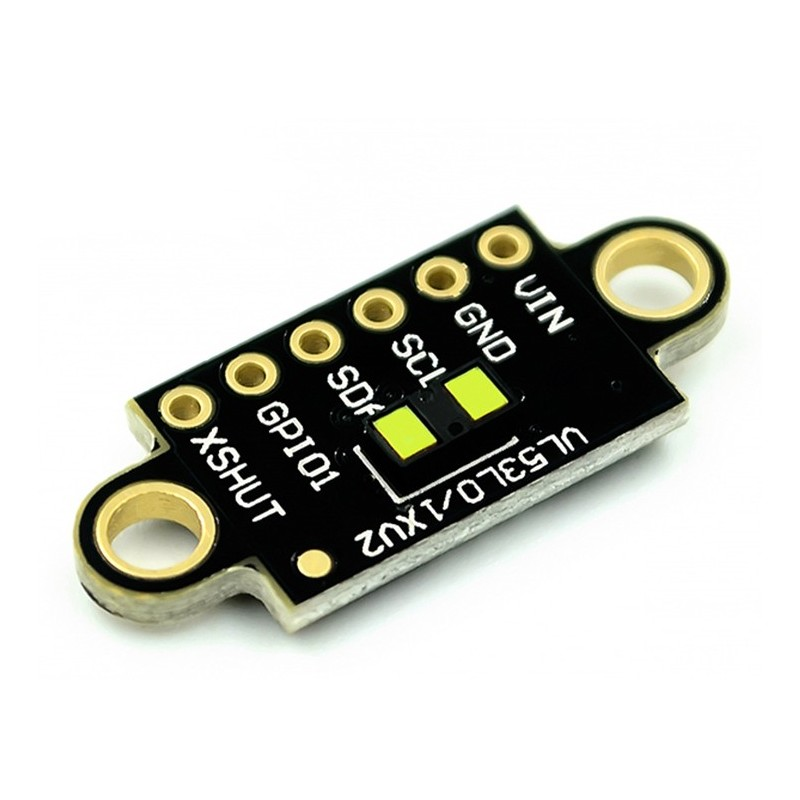
\includegraphics[width=7cm]{includes/images/vl53l1x.jpg}
    \caption{Vzdialenostný senzor VL53L1X}
    \label{fig:vl53l1x}
\end{figure}
\begin{itemize}

    \item Model: VL53L1X

    \item Maximálna vzdialenosť: 400cm

    \item Frekvencia merania: nastaviteľná až do 50Hz

    \item Zorné pole: 27°

    \item Komunikácia: I2C

    \item Odkaz na technický list: \href{https://www.st.com/resource/en/datasheet/vl53l1x.pdf}{Technický list laserového diaľkomera}

\end{itemize}



Na meranie vzdialenosti sme využili štyri takéto moduly pripevnené na dosku vyosené relatívne od dopredného smeru myši o 45° a 10°.

\subsection{PCB}
\subsubsection{Komponenty}
\begin{itemize}
    \item \textbf{Senzory ToF (VL53L1X)}: Prepojenie s ESP32 cez I2C rozhranie.
    \item \textbf{Gyroskop s akcelerometrom (MPU9250)}: Prepojenie s ESP32 cez I2C rozhranie.
    \item \textbf{Driver na motor (TB6612FNG)}: Umiestnený blízko motorov, posiela PWM signály motorom.
    \item \textbf{MCU (ESP32)}: Centrálny riadiaci prvok PCB.
    \item \textbf{Step-up menič na 5V}: Zabezpečenie stabilných 5V pre logické obvody a enkodéry.
    \item \textbf{Logic shifter}: Prekladanie signálov medzi 3,3V a 5V úrovňami.
    \item \textbf{Ochrana batérie}: Meranie napätia batérie a prúdové ochrany.
    \item \textbf{Batéria (Li-ion 1000mAh)}: Umiestnená na PCB s prístupnými napájacími konektormi a ochrannými obvodmi.
\end{itemize}

\subsubsection{Proces tvorby PCB}
\begin{itemize}

\item \textbf{Návrh schémy}\\
Vytvorili sme detailný návrh elektrickej schémy s prepojeniami všetkých komponentov, pričom sme zabezpečili správne napäťové úrovne a prepojenia medzi jednotlivými časťami.

\item \textbf{Rozmiestnenie komponentov}\\
Strategicky sme umiestnili všetky komponenty na PCB tak, aby boli minimalizované rušenia a zohľadnené fyzické rozmery a montážne obmedzenia.

\item \textbf{Vedenie ciest}\\
Navrhnli sme cesty (trasy) pre prepojenie komponentov, s dôrazom na minimalizáciu kríženia ciest a optimalizáciu pre rušenie (napr. použitie samostatných zemných a napájacích rovín).

\item \textbf{Napájanie a ochrany}\\
Implementovali sme obvody na stabilizáciu napätia (3,3V a 5V), ochrany batérie, a zabezpečili, aby boli všetky komponenty správne napájané a chránené.
 
\end{itemize}

\textbf{Taktiež sme museli myslieť na nasledovné:}
\begin{itemize}
    \item Udržanie minimálnej dĺžky kritických signálových trás (I2C, PWM).
    \item Oddelenie silových a signálových ciest na PCB, aby sa minimalizovalo rušenie.
    \item Zabezpečenie dostatočnej kapacity a filtrácie na napájacích cestách.
    \item Implementácia ochranných obvodov pre batériu a citlivé komponenty.
\end{itemize}

\begin{figure}[!htpb]
    \centering
    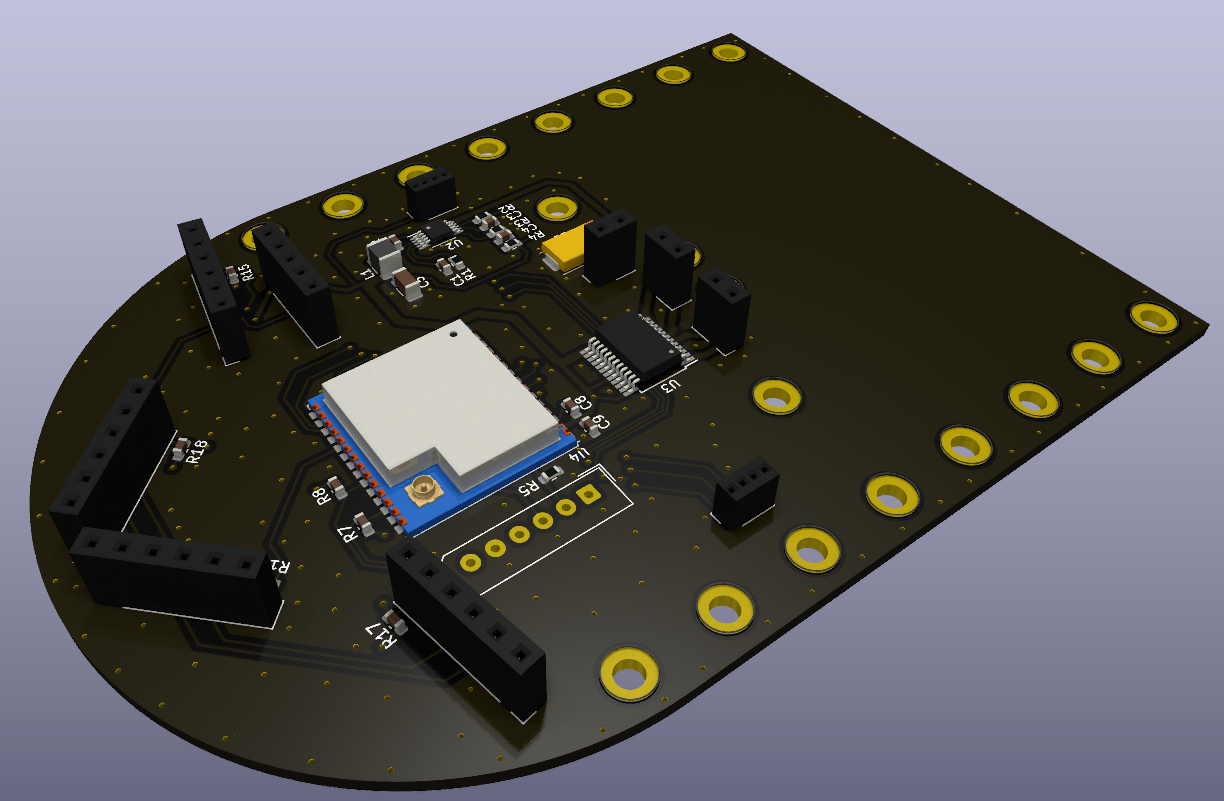
\includegraphics[width=1\linewidth]{includes//images/PCB.png}
    \caption{Návrh PCB dosky použitej vo finálnej verzii.}
    \label{fig:PCB}
\end{figure}

\clearpage\subsection{CAD}
Pri návrhu ako aj pri postupnom iterovaní sme zohľadňovali mnohé aspekty spojené s procesom pri prototypizovaní. Mnohé verzie boli navrhnuté rovnako no v konečnom dôsledku nám ich proces tlače zmenil a museli sme sa s tým vysporiadať, pretože presnosť pri našom návrhu zohrávala kľúčovú úlohu. Pri tlači sme používali dva typy 3D tlače, klasickú FDA no aj živicovú SLA tlač.
\begin{itemize}
\item \textbf{3D návrh kolies}\\
Kolesá pre Micro Mouse boli navrhnuté na základe existujúcich modelov, ktoré poskytli osvedčený základ pre dizajn. Použitie osvedčených modelov umožnilo urýchliť návrhový proces a zaručilo, že výsledné kolesá budú spĺňať požadované špecifikácie.

\item \textbf{Výber modelu}\\
Pre návrh kolies sme vybrali modely, ktoré sú už overené v praxi. Tento prístup minimalizoval riziko návrhových chýb a zabezpečil, že kolesá budú mať vhodné mechanické vlastnosti a správne rozmery.

\item \textbf{Návrh gumy na kolesá}\\
Gumy na kolesá boli použité z existujúceho modelu, čo zabezpečilo optimálnu trakciu a odolnosť. Tento krok eliminoval potrebu vlastného návrhu gumy a umožnil nám sústrediť sa na integráciu kolies do celkového návrhu Micro Mouse.

\item \textbf{3D návrh úchytov}\\
Pre návrh úchytov sme využili iteratívny proces, ktorý umožnil presné prispôsobenie vzdialeností kolies a ich optimálne umiestnenie na Micro Mouse.

\item \textbf{Iteratívny proces návrhu}\\
Návrh úchytov prebiehal v niekoľkých iteráciách, pričom sme upravovali vzdialenosti kolies a ich polohu, aby sme dosiahli najlepšiu možnú stabilitu a pohyblivosť Micro Mouse. Tento proces zahŕňal testovanie rôznych konfigurácií a úpravou návrhu na základe výsledkov týchto testov.

\item \textbf{Optimalizácia vzdialeností}\\
Upravovanie vzdialeností kolies bolo kľúčové pre dosiahnutie optimálnej manévrovateľnosti. Iteratívne úpravy umožnili presné doladenie návrhu, čo viedlo k zlepšeniu celkového výkonu Micro Mouse.
\end{itemize}
\clearpage Návrh a výroba 3D komponentov pre Micro Mouse zahŕňala použitie existujúcich modelov kolies a gumy, ako aj iteratívny návrh úchytov. Tento prístup umožnil efektívne vytvorenie funkčných a spoľahlivých komponentov, ktoré prispievajú k optimálnemu výkonu Micro Mouse.

\begin{figure}[!htpb]
    \centering
    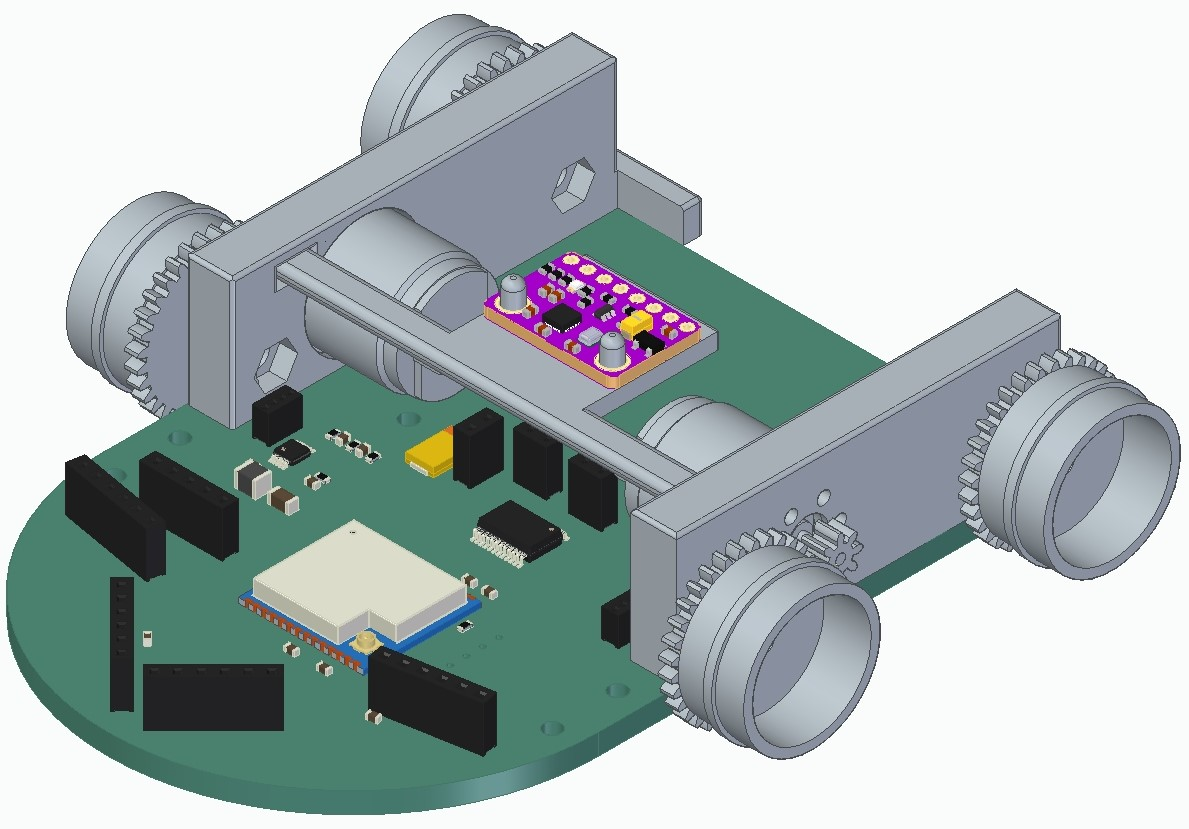
\includegraphics[width=1\linewidth]{includes//images/main_board.jpg}
    \caption{Konečná verzia návrhu všetkých komponentov vyrábaných pomocou 3D tlače usporiadaných na PCB.}
    \label{fig:MainBoard}
\end{figure}

\section{Software}
\label{sec:software}

Na písanie kódu sme použili prostredie \textbf{esp\_idf} verzie \textit{4.4.7}, ktoré sme vytvorili za~pomoci
ich repozitára \cite{espGithub}.

Postup na~inicializáciu ESP IDF a~následné spustenie projektu je nasledovný:
\begin{enumerate}
	\item Stiahnutie ESP IDF z~repozitára \cite{espGithub} (My sme použili verziu 4.4.7).
	\item Spustenie príkazu \textit{./install.sh esp32} pre~Linux.
		Tento príkaz stiahne a~nainštaluje všetky potrebne závislosti.
	\item Exportovanie súboru \textit{. ./export.sh} pre~Linux.
		Tento príkaz nastaví všetky potrebne premenne prostredia.
	\item Zmeniť aktuálny adresár na~náš projekt.
	\item Spustiť príkaz \textit{idf.py build} pre~kompiláciu projektu.
	\item Spustiť príkaz \textit{idf.py -P <PORT\_NR> flash} pre~nahratie binárneho súboru do~ESP32.
		Pre tuto operáciu je potrebne mať pripojený počítač a~misku cez UART.
	\item Spustiť príkaz \textit{idf.py monitor} pre~sledovanie výstupu z~ESP32.
\end{enumerate}

Alternatívne spustenie je možné pomocou platformy \textbf{Visual Studio Code} s~nainštalovaným rozšírením
\textbf{ESP-IDF}~\cite{espIDF}.
\newpage
\subsection{Senzory}
\subsubsection{VL53L1X}
Pre snímanie vzdialenosti bola vytvorená knižnica na kalibráciu a vyčítavanie dát zo senzora VL53L1X. Komunikácia prebieha prostredníctvom komunikačného protokolu $I^2 C$. Knižnica je nadstavbou nad voľne dostupným rozhraním od STMicroelectronics.
\begin{figure}[!htpb]
    \centering
    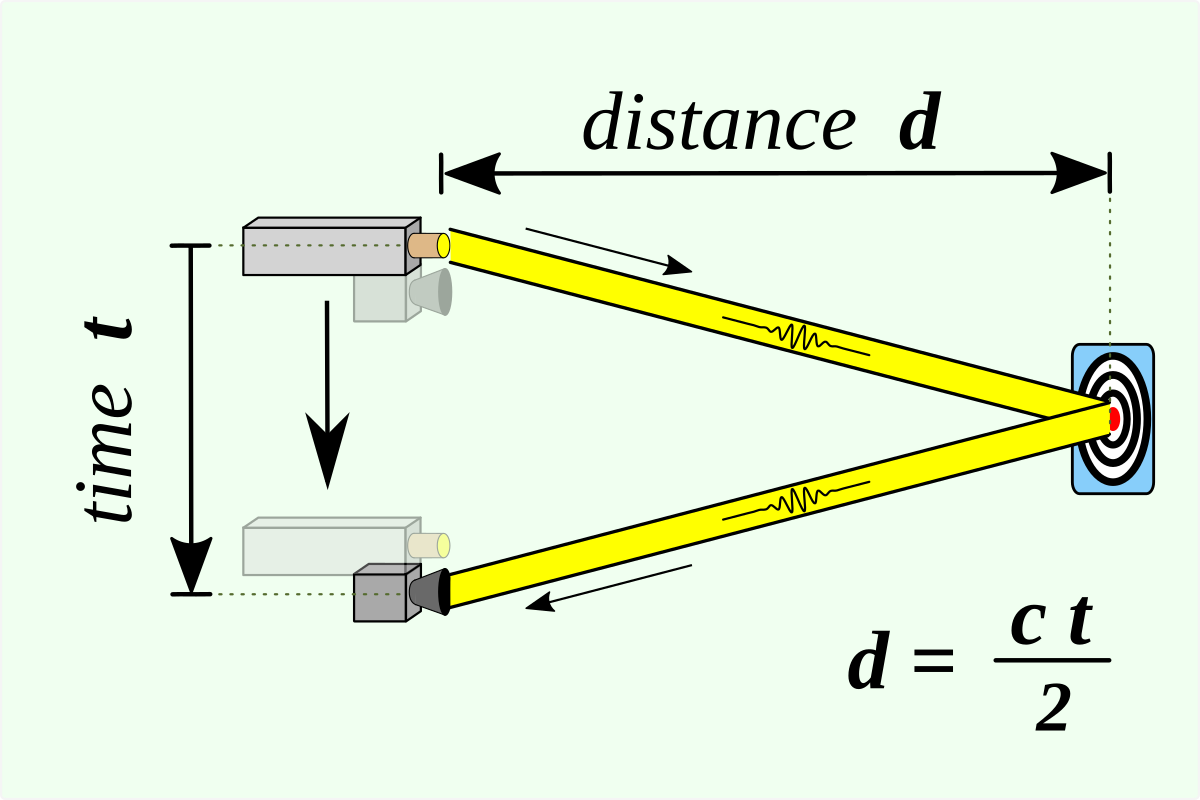
\includegraphics[width=8cm]{includes//images/tof_pic.png}
    \caption{Základný princíp ToF}
    \label{fig:tof_pic}
\end{figure}
Na obrázku \ref{fig:tof_pic} je zobrazený princíp fungovania senzora využívajúceho metódu Time-of-Flight (ToF) pre meranie vzdialenosti. Zariadenie emituje svetelný signál, ktorý sa odrazi od objektu a vráti späť k senzoru.
\subsubsection{MPU9250}
\begin{figure}[!htpb]
    \centering
    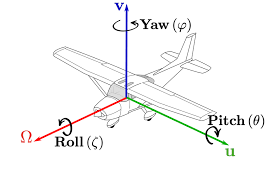
\includegraphics[width=10cm]{includes//images/rpy.png}
    \caption{Gyroskop s akcelerometrom MPU9250 }
    \label{fig:rpy}
\end{figure}
V našom projekte sme použili senzor MPU9250, ktorý je trojosovým akcelerometrom a gyroskopom. Tento senzor nám umožňuje získavať presné údaje o orientácii mikromyši v trojrozmernom priestore. Kľúčovou súčasťou spracovania dát z tohto senzoru je výpočet Eulerových uhlov -- roll, pitch a yaw. Tieto údaje sú neoceniteľné pre stabilizáciu a presné navigačné manévre mikromyši, poskytujúc tak lepší prehľad o jej aktuálnom náklone a orientácii.

\subsubsection{IEH2-4096}
%TODO: enkodery - inkrementalne, mame vytvoreny impulz counter, ktory nam vrati interrupt po 1/8 natocenia motora -- kazdu 1/8 otocenia motora = tick, prepocitame si to ---- Poprosim skontrolovat
V rámci nášho projektu sme implementovali impulzové čítače s inkrementálnymi enkodérmi IEH2-4096, ktoré sú pripevnené na motory. Tieto enkodéry generujú signál v podobe elektrických impulzov v závislosti od uhlového pohybu motorov. Pre naše účely sme nastavili systém tak, aby generoval prerušenie po každej 1/8 otáčke motora.

Každý "tick" nám indikuje 1/8 otáčky motora, a pomocou softvéru potom prepočítavame tieto hodnoty na požadované metrické jednotky (napríklad stupne alebo radiány). Tento mechanizmus nám umožňuje presne sledovať a regulovať pohyb mikromyši, čo je kritické pre presné navigačné a kontrolné úlohy v autonómnych aplikáciách.
\newpage
\subsection{Odometria}
\label{subsec:odometria}

% Pridat referencia na~motor a~enkoder ked budu vytvorene v~hardweri
Pri počítaní polohy robota bola použítá odometria.
Použili sme na~to inkrementálny enkóder \ref{encoder_section}, ktorý je pripojený na~motor \ref{motor_section}. Z enkóderov si získame aktuálnu polohu robota
cez základný vzťah:

\begin{equation}
	\label{eq:odometria}
	 \Delta x_t = x_{t-1} + \Delta s_t \cdot \cos(\phi_{t-1} + \Delta \phi_t)
\end{equation}
\begin{align}
	\Delta y_t = y_{t-1} + \Delta s_t \cdot \sin(\phi_{t-1} + \Delta \phi_t)
\end{align}
,kde:
\begin{itemize}
    \item $\Delta x_t$ a $\Delta y_t$ sú zmeny pozície robota v osiach $x$ a $y$ v čase $t$,
    \item $x_{t-1}$ a $y_{t-1}$ sú predchádzajúce pozície robota v osiach $x$ a $y$,
    \item $\Delta s_t$ je vzdialenosť, ktorú robot prešiel od posledného merania,
    \item $\phi_{t-1}$ je predchádzajúci uhol orientácie robota,
    \item $\Delta \phi_t$ je zmena uhla orientácie robota získaná z gyroskopu.
\end{itemize}

Pre lepšie pochopenie odometrie a jej presnosti je dôležité zvážiť aj potenciálne chyby z enkóderov a gyroskopu, ako aj spôsoby ich korekcie v softvérovom riešení robota.


\newpage

\subsection{PID regulátor motorov}
\label{subsec:pid}

Do motorov posielame ako akčný zásah signál PWM (\acrlong{PWM}). Tento signál môže nadobúdať hodnoty od~0 po~1023.
Zároveň musíme myslieť aj na~prepäťovú ochranu. Keď pošleme do~motorov veľké zrýchlenie, tak sa stane, že sa program
na~čipe zresetuje.

Aby sme ošetrili tieto situácie, sme pridali rozbehový člen v podobe rampového signálu, ktorý zabezpečí postupné zmeny žiadanej hodnoty namiesto skokových zmien. Na riadenie motorov sme implementovali PID regulátor s Antiwindupom. 
Jeho obmedzenie je nastavené zdola na~0 a~zhora na~1023. Toto obmedzenie zdola je nastavené na~0 kvôli implementácii nastavenia smeru
otáčania motorov. V~prostredí ESP musíme dopredu nastaviť smer otáčania motorov. Po jeho nastavení sa všetky hodnoty
posielajú ako \textit{unsigned}. Teda ak by sme mu poslali zápornú hodnotu, tak by sa motor rozbehol nastaveným smerom.
Antiwindup zapojenie maximálnu rýchlosť obmedzuje na~1023.

Pre jednoduchosť ovládania sme nastavili regulátor tak, aby vstupná žiadaná hodnota bol v~milimetroch za~sekundu.
Regulátor si túto hodnotu prepočíta na~PWM signál, ktorý pošle motorom. Spätné väzby sa získavajú z~enkóderov
a~dopočítavajú sa na~milimetre za~sekundu. Tieto hodnoty sa taktiež prepočítajú na~PWM signál. Prepočet z~milimetrov
za sekundu na~PWM signál je závislý uskutočňovaný nasledujúcim výpočtom:

\begin{equation}
	\text{PWM} = d \pi \frac{IMP_t}{IMP_{pr} i \Delta t}
	\label{eq:mmps2pwm}
\end{equation}

Rovnica \ref{eq:mmps2pwm} obsahuje parametre:
\begin{itemize}
	\item d - Priemer kolesa,
	\item $IMP_t$ - Aktuálne impulzy z~enkóderu,
	\item $IMP_{pr}$ - Impulzy z~enkóderu za~jednu otáčku (per rotation),
	\item i - Pomer prevodovky motora. Na~našich motoroch je to prevod 32:8,
	\item $\Delta t$ - Časový interval od~posledného merania
\end{itemize}

\newpage
\subsection{Riadiaci algoritmus}
%TODO: UML Algoritmus, popisat k nemu veci ----- ak budete chciet menit veci v diagrame, v images bude aj .drawio file, ktory sa da rovno editovat pre usetrenie casu
\begin{figure}[!htpb]
    \centering
    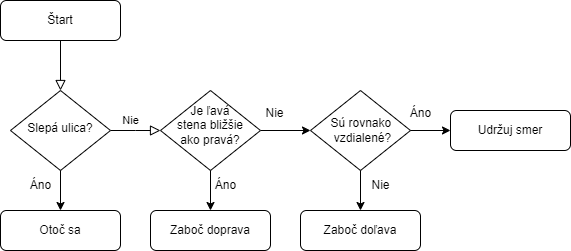
\includegraphics[width=1\linewidth]{includes//images/uml_algo.png}
    \caption{UML diagram logiky algoritmu }
    \label{fig:uml_algo}
\end{figure}
Na obrázku \ref{fig:uml_algo} je znázornený tokový diagram, ktorý predstavuje algoritmus na rozhodovanie o pohybe v priestore. Tento diagram obsahuje niekoľko krokov a rozhodnutí:
\begin{enumerate}
    \item \textbf{Štart - }Začiatočný bod algoritmu.
    \item \textbf{Slepá ulica? - }Rozhodovací krok, kde sa algoritmus pýta, či sa pred myškou nachádza slepá ulica.
        \begin{itemize}
            \item Ak \textbf{áno}, nasleduje krok Otoč sa, čo znamená zmenu smeru o 180 stupňov.
            \item Ak \textbf{nie}, pokračuje ďalším rozhodnutím.
        \end{itemize}
    \item \textbf{Je ľavá stena bližšie ako pravá? - }Ďalšie rozhodovacie kritérium zvažujúce relatívne pozície stien.
        \begin{itemize}
            \item Ak \textbf{áno}, nasleduje krok Zaboč doprava.
            \item Ak \textbf{nie}, presmeruje sa na ďalší rozhodovací bod.
        \end{itemize}
    \item \textbf{Sú rovnako vzdialené? - }Rozhoduje, či sú obidve steny rovnako vzdialené od myšky.
        \begin{itemize}
            \item Ak \textbf{áno}, nasleduje krok Zaboč doľava.
            \item Ak \textbf{nie}, vykoná sa krok Udržuj smer, čo znamená pokračovanie v súčasnom smere bez zmeny.
        \end{itemize}
\end{enumerate}
\subsection{UDP Komunikácia}
\subsubsection{Client}
Klientom v našom prípade je ESP32, ktorý sa používa v PCB mikromyši. Toto zariadenie je zodpovedné za zber údajov o stave a správaní mikromyši a ich odosielanie na server. Komunikácia s serverom prebieha prostredníctvom UDP protokolu, čo umožňuje rýchly a efektívny prenos dát.
\subsubsection{Server}
Na strane servera sme použili vývojové prostredie Qt Creator s programovacím jazykom C++ na implementáciu serverovej časti, ktorá prijíma dáta od klienta. Server je integrovaný s mini HMI (Human-Machine Interface) aplikáciou, ktorá umožňuje real-time vizualizáciu dát prostredníctvom grafov a poskytuje užívateľské rozhranie pre sledovanie a ladenie správania mikromyši.

\begin{figure}[!htpb]
    \centering
    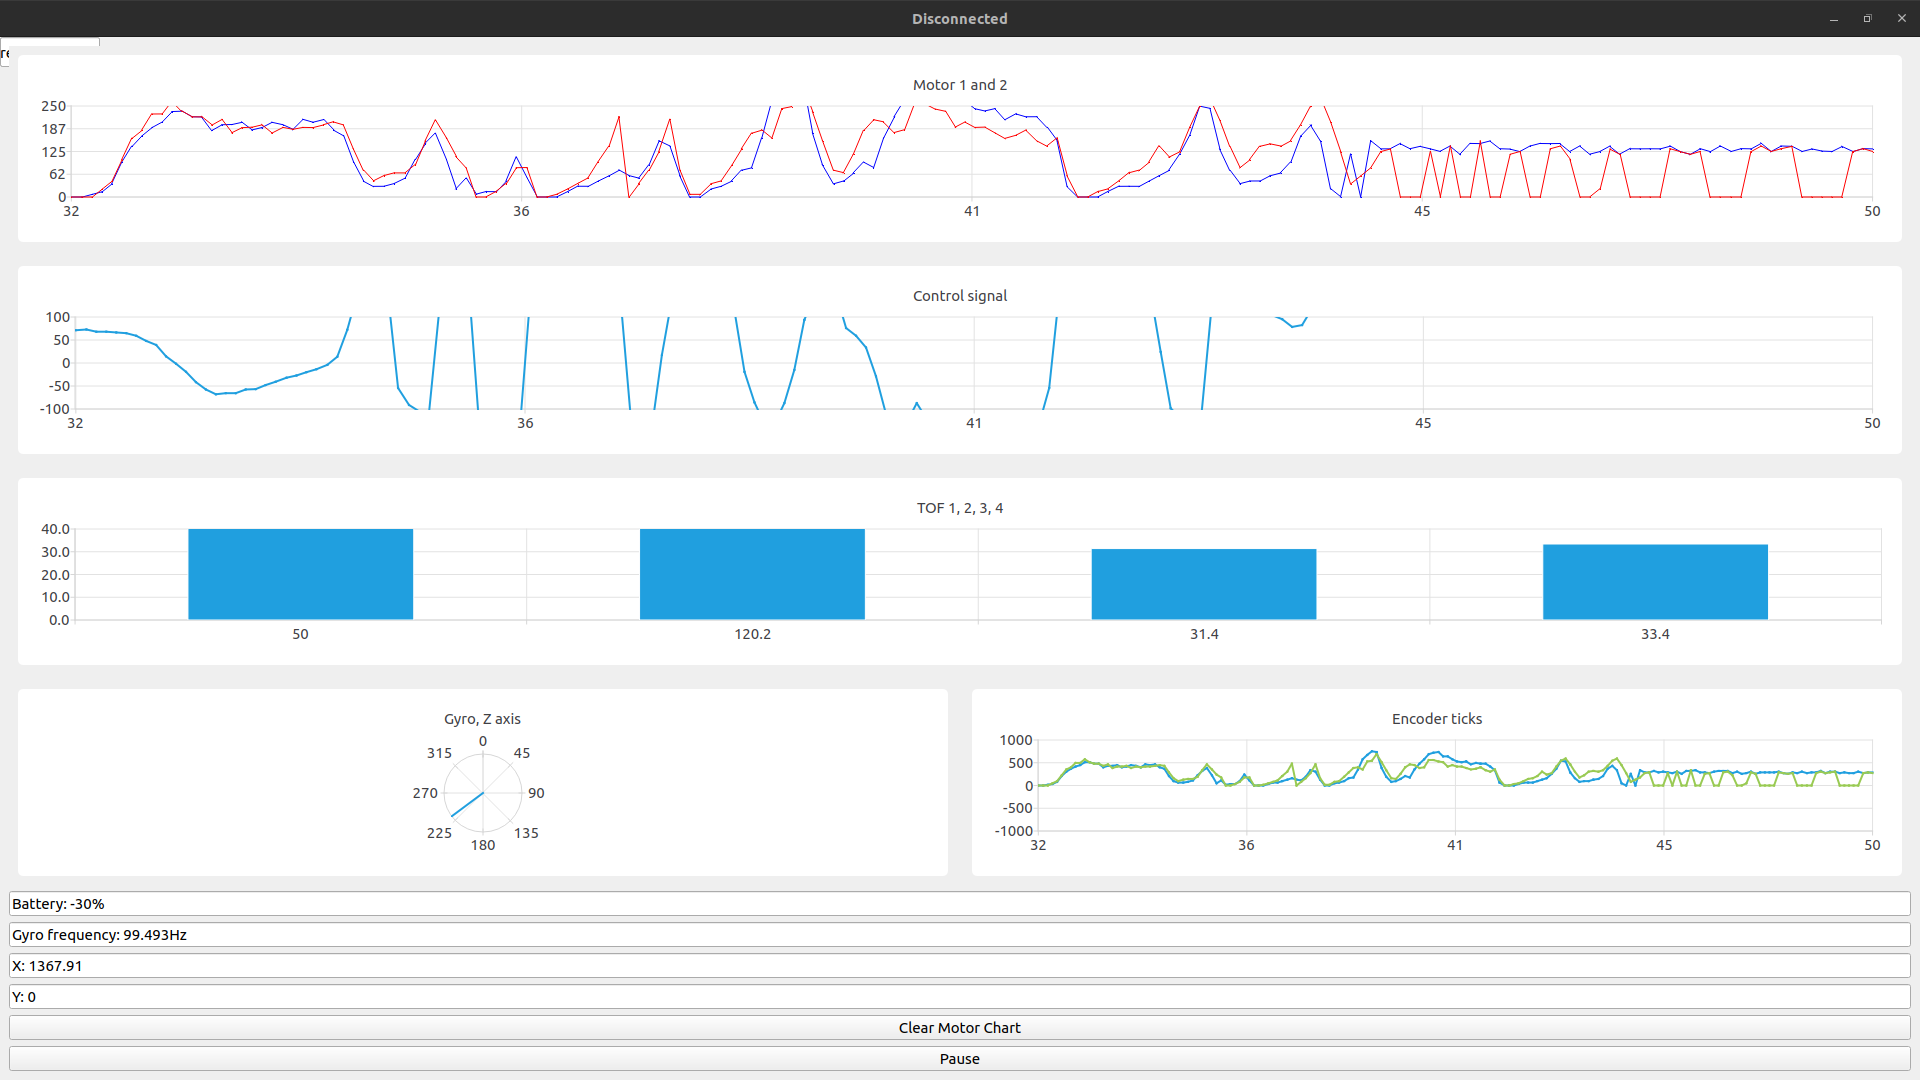
\includegraphics[width=14cm]{includes//images/image.png}
    \caption{Používateľské rozhranie HMI aplikácie }
    \label{fig:UDP}
\end{figure}
HMI aplikácia je kľúčovým nástrojom pre efektívne diagnostikovanie a optimalizáciu výkonu autonómnej mikromyši. \ref{fig:UDP} 